\section{Auswertung der Regleroptimierung am DC-Motor}
\subsection{Synthetisierte Regler}

% tripple minipage
\begin{figure}[H]
    \centering
    \begin{minipage}[t]{0.32\textwidth}
        \begin{table}[H]
            \center
            \begin{tabular}{@{}cr@{}}
                    \toprule
                    \textbf{Parameter}              & \textbf{Wert} \\
                    \midrule
                    $Kp$                            & 11.1112 \\[0.5ex]
                    $Ki$                            & 79.365 \\[0.5ex]
                    $Kd$                            & -1.8759e-4 \\[0.5ex]
                    $Kn$                            & 0.50616 \\[0.5ex]
                    \textbf{Konstante}              & \textbf{Wert} \\
                    $u_\mathbf{satHigh}$            & 10 \\[0.5ex]
                    $u_\mathbf{satLow}$             & 0 \\[0.5ex]
                    $I_{\mathbf{SatHigh}}$          & 10 \\[0.5ex]
                    $I_{\mathbf{SatLow}}$           & -10 \\[0.5ex]
                    Anti-Windup                     & Clamping \\[0.5ex]
                    \bottomrule
            \end{tabular}
            \caption{Reglerparameter des mit \textit{systune} optimierten Reglers}
            \label{tab:SimpleMotorSystune_OptimizationParameters}
        \end{table}
    \end{minipage}
    \hfill
    \begin{minipage}[t]{0.32\textwidth}
        \begin{table}[H]
            \center
            \begin{tabular}{@{}cr@{}}
                    \toprule
                    \textbf{Parameter}              & \textbf{Wert} \\
                    \midrule
                    $Kp$                            & 6.62 \\[0.5ex]
                    $Ki$                            & 109 \\[0.5ex]
                    $Kd$                            & 0 \\[0.5ex]
                    $Kn$                            & 0 \\[0.5ex]
                    \textbf{Konstante}              & \textbf{Wert} \\
                    $u_\mathbf{satHigh}$            & 10 \\[0.5ex]
                    $u_\mathbf{satLow}$             & 0 \\[0.5ex]
                    $I_{\mathbf{SatHigh}}$          & 10 \\[0.5ex]
                    $I_{\mathbf{SatLow}}$           & -10 \\[0.5ex]
                    Anti-Windup                     & Clamping \\[0.5ex]
                    \bottomrule
            \end{tabular}
            \caption{Reglerparameter des mit \gls{GA} optimierten Reglers}
            \label{tab:SimpleMotorGA_OptimizationParameters}
        \end{table}
    \end{minipage}
    \hfill
    \begin{minipage}[t]{0.32\textwidth}
        \begin{table}[H]
            \center
            \begin{tabular}{@{}cr@{}}
                    \toprule
                    \textbf{Parameter}              & \textbf{Wert} \\
                    \midrule
                    $Kp$                            & 5.7 \\[0.5ex]
                    $Ki$                            & 84.5 \\[0.5ex]
                    $Kd$                            & -0.488 \\[0.5ex]
                    $Kn$                            & 0.625 \\[0.5ex]
                    \textbf{Konstante}              & \textbf{Wert} \\
                    $u_\mathbf{satHigh}$            & 10 \\[0.5ex]
                    $u_\mathbf{satLow}$             & 0 \\[0.5ex]
                    $I_{\mathbf{SatHigh}}$          & 10 \\[0.5ex]
                    $I_{\mathbf{SatLow}}$           & -10 \\[0.5ex]
                    Anti-Windup                     & Clamping \\[0.5ex]
                    \bottomrule
            \end{tabular}
            \caption{Reglerparameter des mit \gls{DE} optimierten Reglers}
            \label{tab:SimpleMotorDE_OptimizationParameters}
        \end{table}
    \end{minipage}
\end{figure}

\subsection{Systemverhalten am realen Prozess}
\begin{figure}[H]
	\center
    %\vspace{-1.6cm}
    \includegraphics[width=\linewidth]{images/SimpleMotor/CombinedMethodes_realResult.pdf}
    \caption{Kombinierte Antwort auf Stimulation der optimierten Regler am DC-Motor}
    \label{fig:SimpleMotorCombinedMethodes_realResult}
\end{figure}

\definecolor{systuneColor}{HTML}{3189f5}
\definecolor{geneticColor}{HTML}{2cf533}
\definecolor{differentialColor}{HTML}{cc2cf5}
\minipagedOrBelowEachOther
{
    In \ref{fig:SimpleMotorCombinedMethodes_realResult} ist die Antwort auf die Stimulationssignale
    der drei Systeme dargestellt. Das Signal $r$ ist die Ziel-Drehzahl und 
    $l$ stellt die Störgrösse dar. 
}{}

\minipagedOrBelowEachOther
{    
    \subparagraph{\textcolor{systuneColor}{\textit{Systune} Regler}}
        \noindent
        \\
        Der mit \textit{systune} optimierte Regler zeigt ein stärkeres Rauschverhalten als die anderen beiden Regler.

        
    \subparagraph{\textcolor{geneticColor}{Genetisch optimierter Regler}}
        \noindent
        \\
        Der mit dem \gls{GA} optimierte Regler zeigt ein schnelleres Verhalten als der \textit{systune} Regler
}
{
	\subparagraph{\textcolor{differentialColor}{Differential Evolution optimierter Regler}}
        \noindent
        \\
        Der mit dem \gls{DE} optimierte Regler zeigt ein ziemlich ähnliches Verhalten wie 
        der Genetisch optimierte Regler. Er hat jedoch ein etwas höheres Überschwingen.
        Die Rauschunterdrückung ist bei diesem Regler am besten.
}

\newpage
\subsection{Lernverlauf}
\begin{figure}[H]
	\center
    %\vspace{-1.6cm}
    \includegraphics[width=\linewidth]{images/SimpleMotor/CombinedMethodes_Simulation_LearningHistory_1.pdf}
    \caption{Lernverlauf der kombinierten Optimierungsmethoden (GA + DE)}
    \label{fig:SimpleMotorCombinedMethodes_Simulation_LearningHistory_1}
\end{figure}

\minipagedOrBelowEachOther
{
    In~\ref{fig:SimpleMotorCombinedMethodes_Simulation_LearningHistory_1} ist der Lernverlauf
    der beiden Methoden \gls{GA} und \gls{DE} übereinandergelegt dargestellt. Der Vergleich zeigt, 
    beide Methoden sind in der Lage das gleiche Optimum zu finden.
    Der DE konvergiert dabei etwas schneller als der GA, hat aber das Problem, 
    dass in dem Test 9 von 10 Durchläufen nicht das bessere Optimum gefunden wurde.
}
{
    Der GA hat deutlich länger um das bislang beste Ergebnis des DE zu erreichen,
    schafft es aber in allen 10 Durchläufen eine bessere Lösung zu finden als der DE in 9 von 10 Durchläufen.	
}

\horizontalLine
\minipagedOrBelowEachOther
{
    Der Lernverlauf ist leider für den \textit{systune} Regler nicht verfügbar, 
    damit dennoch ein Vergleich möglich ist wendet man die vom \textit{systune} berechneten Reglerparameter in der
    Simulationssoftware an und misst den Fehler mit der gleichen Bewertungsfunktion wie bei den anderen beiden Methoden.
    \textit{Systune} erreicht mit den in~\fullref{tab:SimpleMotorSystune_OptimizationParameters} angegebenen Parametern
    einen Fehler von $5.06624$.
    % Params:
    % Kp = 11.1112;
    % Ki = 79.365;
    % Kd = -1.8759e-4;
    % Tf = 1.9757;
    % Integral Saturation High = 10;
    % Integral Saturation Low = -10;
    % Output Saturation High = 10;
    % Output Saturation Low = 0;
    %
    % Scores:
    % Score Component:  0.99494
    % Score Component:  3.71835
    % Score Component:  0.352946
    % Score Component:  0
    % Score Component:  0
    % Custom PID Test Score:  5.06624

    
}
{
    \textit{Systune} hat mit $5.06624$ einen höheren Fehler als beide anderen Methoden erreicht.
    Dies liegt sehr wahrscheinlich daran, dass die Optimierungskriterien von \textit{systune} nicht exakt mit der Bewertungsfunktion
    der Simulationssoftware übereinstimmen.\\


    Eine weitere Vermutung ist, dass die Methoden GA und DE eine bessere Lösung finden, 
    weil sie auch an nichtlinearen Systemen angewendet werden und sich dadurch 
    besser auf die nichtlinearen Effekte, wie die vorhandenen Sättigungen und den Anti-Windup, anpassen können.

    
}



\newpage
\subsection{Frequenzanalyse der optimierten Regler}
% === systunePID Performance ===
% Rise Time:        0.031 s
% Settling Time:    0.055 s
% Overshoot:        0.00 %
% 
% Gain Margin:    Inf dB
% Phase Margin:     90.00 °
% 
% === geneticPID Performance ===
% Rise Time:        0.035 s
% Settling Time:    0.183 s
% Overshoot:        6.76 %
% 
% Gain Margin:    Inf dB
% Phase Margin:     80.83 °
% 
% === differentialPID Performance ===
% Rise Time:        0.043 s
% Settling Time:    0.207 s
% Overshoot:        6.81 %
% 
% Gain Margin:    Inf dB
% Phase Margin:     79.97 °

%\horizontalLine
\minipagedOrBelowEachOther
{
    \vspace{0.6cm}
    Im \ref{fig:SimpleMotorCombinedMethodes_PIDBode} sind die Bode-Diagramme der drei optimierten Regler dargestellt.
    Diese Zeigen die Frequenzgänge der Regler ohne die Regelstrecke.
    Es ist zu erkennen, dass die Regler die Phase auf 0° anheben und 
    die Verstärkung für kleine Frequenzen sehr hoch ist.
    Alle drei Regler zeigen kein striktes Tiefpassverhalten. Frequenzen ab 10rad/s werden nicht weiter gedämpft.
}
{
    \begin{figure}[H]
        \center
        %\vspace{-1.6cm}
        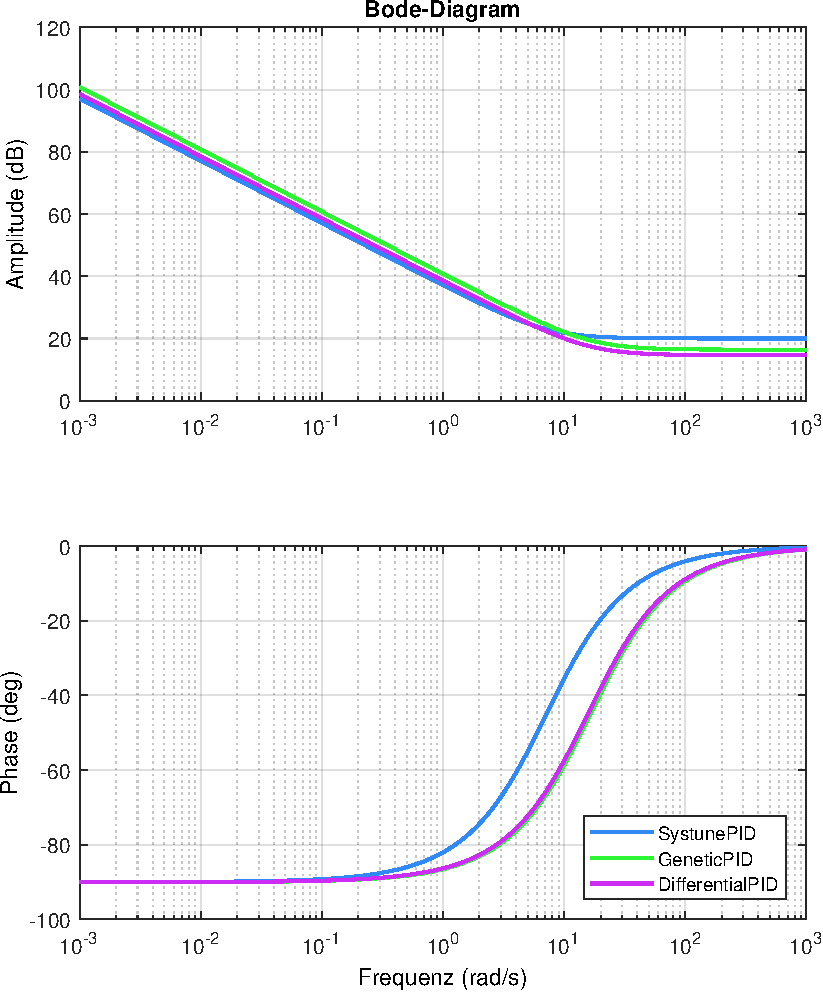
\includegraphics[width=\linewidth]{images/SimpleMotor/CombinedMethodes_PIDBode.pdf}
        \caption{Bode-Diagramm der optimierten Regler}
        \label{fig:SimpleMotorCombinedMethodes_PIDBode}
    \end{figure}
}


\newpage
\subsection{Frequenzanalyse der optimierten Systeme}
%\horizontalLine
\minipagedOrBelowEachOther
{
    \begin{figure}[H]
        \center
        %\vspace{-1.6cm}
        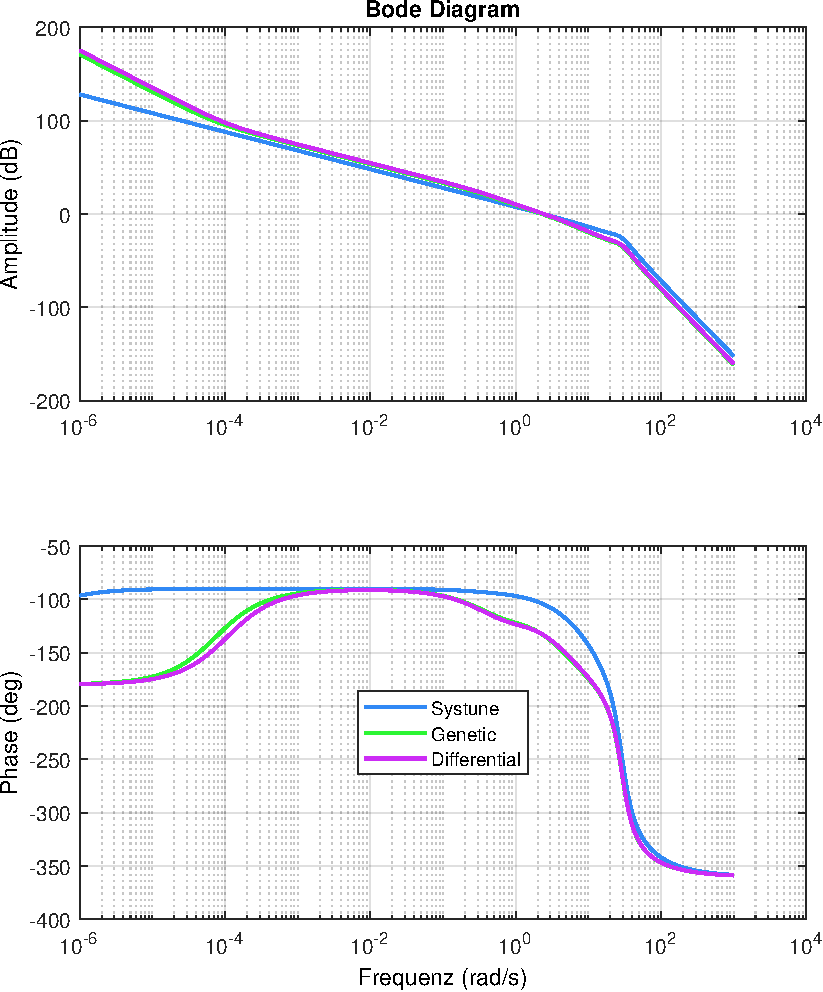
\includegraphics[width=\linewidth]{images/SimpleMotor/CombinedMethodes_SystemBode.pdf}
        \caption{Bode-Diagramm der optimierten Vorwärts Pfade der einzelnen Systeme}
        \label{fig:SimpleMotorCombinedMethodes_SystemBode}
    \end{figure}
    Das Bode-Diagramm in~\ref{fig:SimpleMotorCombinedMethodes_SystemBode} und das
    Nyquist-Diagramm in~\ref{fig:SimpleMotorCombinedMethodes_SystemLogScaleNyquist} zeigen,
    jeweils die Frequenzgänge der optimierten Vorwärts Pfade der drei Systeme:
    \begin{itemize}
        \item \textcolor{systuneColor}{$PID_{\mathbf{systune}} \cdot MotorSystem$}
        \item \textcolor{geneticColor}{$PID_{\mathbf{genetic}} \cdot MotorSystem$}
        \item \textcolor{differentialColor}{$PID_{\mathbf{differential}} \cdot MotorSystem$}
    \end{itemize}

    Im Bode-Diagramm fällt auf, dass der Regler von \textit{systune} nicht zusätzliche Phase klaut.
    Die beste Rauschunterdrückung bietet jedoch der Regler von Differential Evolution.
    
    
}
{
    \begin{figure}[H]
        \center
        %\vspace{-1.6cm}
        \includegraphics[width=\linewidth]{images/SimpleMotor/CombinedMethodes_SystemLogScaleNyquist.pdf}
        \vspace{-0.18cm}
        \caption{Logarithmisches Nyquist-Diagramm der optimierten Vorwärts Pfade der einzelnen Systeme \cite{matlabScriptNyquistLog}}
        \label{fig:SimpleMotorCombinedMethodes_SystemLogScaleNyquist}
    \end{figure}

    \begin{table}[H]
        \center
        \begin{tabular}{@{}cr@{}}
                \toprule
                \textbf{Phasenreserve}              & \textbf{Wert} \\
                \midrule
                \textcolor{systuneColor}{\textit{Systune}}                          & 90.00 ° \\[0.5ex]
                \textcolor{geneticColor}{Genetisch}                        & 80.83 ° \\[0.5ex]
                \textcolor{differentialColor}{Differential Evolution}           & 79.97 ° \\[0.5ex]
                \hline
                \textbf{Verstärkungsreserve}              &  \\
                \hline
                \textcolor{systuneColor}{\textit{Systune}}                          & Inf dB \\[0.5ex]
                \textcolor{geneticColor}{Genetisch}                        & Inf dB \\[0.5ex]
                \textcolor{differentialColor}{Differential Evolution}           & Inf dB \\[0.5ex]
                \bottomrule
        \end{tabular}
        \caption{Reserven optimierten Systeme}
        \label{tab:SimpleMotorCombinedMethodes_AnalyzedData}
    \end{table}
}


\newpage
\subsection{Stabilitätsanalyse der optimierten Systeme}
\subsubsection{Sensitivität}
\begin{figure}[H]
    %\vspace{-1.6cm}
    \includegraphics[width=\linewidth]{images/SimpleMotor/CombinedMethodes_Sensitivity.pdf}
    \caption{Sensitivität der optimierten Systeme}
    \label{fig:SimpleMotorCombinedMethodes_Sensitivity}
\end{figure}
\minipagedOrBelowEachOther
{
    Das Sensitivitäts-Diagramm in \ref{fig:SimpleMotorCombinedMethodes_Sensitivity} zeigt,
    für alle drei Systeme einen ähnlichen Verlauf. Keine Überhöhung, was ein gutes Stabilitätsverhalten andeutet.
    Nicht auf den ersten Blick ersichtlich ist jedoch, dass die Systeme sehr empfindlich auf Totzeiten reagieren.
    Dies ist in Abschnitt \fullref{sec:SimpleMotorStabilityDelayMarginsPlot} dargestellt.
}
{

}

\horizontalLine
\begin{figure}[H]
    \subsubsection{Phasen- \& Verstärkungsreserve Diagramme der optimierten Systeme}
    \begin{minipage}[t]{0.32\textwidth}
        \begin{figure}[H]
            %\vspace{-1.6cm}
            \includegraphics[width=\linewidth]{images/SimpleMotor/SystuneStabilityPhaseMarginsPlot.pdf}
            \caption{Phasen- \& Verstärkungsreserve des mit \textit{systune} optimierten Systems}
            \label{fig:SimpleMotorSystuneStabilityPhaseMarginsPlot}
        \end{figure}
    \end{minipage}
    \hfill
    \begin{minipage}[t]{0.32\textwidth}
        \begin{figure}[H]
            %\vspace{-1.6cm}
            \includegraphics[width=\linewidth]{images/SimpleMotor/GeneticStabilityPhaseMarginsPlot.pdf}
            \caption{Phasen- \& Verstärkungsreserve des mit Genetic optimierten Systems}
            \label{fig:SimpleMotorGeneticStabilityPhaseMarginsPlot}
        \end{figure}
    \end{minipage}
    \hfill
    \begin{minipage}[t]{0.32\textwidth}
        \begin{figure}[H]
            %\vspace{-1.6cm}
            \includegraphics[width=\linewidth]{images/SimpleMotor/DifferentialStabilityPhaseMarginsPlot.pdf}
            \caption{Phasen- \& Verstärkungsreserve des mit Differential Evolution optimierten Systems}
            \label{fig:SimpleMotorDifferentialStabilityPhaseMarginsPlot}
        \end{figure}
    \end{minipage}


\minipagedOrBelowEachOther
{
    Die drei Diagramme in
\ref{fig:SimpleMotorSystuneStabilityPhaseMarginsPlot}, 
\ref{fig:SimpleMotorGeneticStabilityPhaseMarginsPlot} und 
\ref{fig:SimpleMotorDifferentialStabilityPhaseMarginsPlot}
    zeigen die detaillierten Stabilitätsreserven als Kombination von Verstärkung und 
    konstanter Phasenverschiebung.
    Wie diese Diagramme zu lesen sind, ist in folgendem Kapitel erklärt:\\
\fullref{sec:StabilitaetsPhaseMarginPlot}
}
{
    Das System welches mit \textit{systune} optimiert wurde, zeigt eine grössere Fläche indem das System stabil bleibt.
    Dies deutet darauf hin, dass dieses System robuster gegenüber Verstärkungsänderungen und Phasenverschiebungen ist.
}
\end{figure}



\newpage
\begin{figure}[H]
    \subsubsection{Totzeit- \& Verstärkungsreserve Diagramme der optimierten Systeme}
    \label{sec:SimpleMotorStabilityDelayMarginsPlot}
    \begin{minipage}[t]{0.32\textwidth}
        \begin{figure}[H]
            %\vspace{-1.6cm}
            \includegraphics[width=\linewidth]{images/SimpleMotor/SystuneStabilityDelayMarginsPlot.pdf}
            \caption{Totzeit- \& Verstärkungsreserve des mit \textit{systune} optimierten Systems}
            \label{fig:SimpleMotorSystuneStabilityDelayMarginsPlot}
        \end{figure}
    \end{minipage}
    \hfill
    \begin{minipage}[t]{0.32\textwidth}
        \begin{figure}[H]
            %\vspace{-1.6cm}
            \includegraphics[width=\linewidth]{images/SimpleMotor/GeneticStabilityDelayMarginsPlot.pdf}
            \caption{Totzeit- \& Verstärkungsreserve des mit Genetic optimierten Systems}
            \label{fig:SimpleMotorGeneticStabilityDelayMarginsPlot}
        \end{figure}
    \end{minipage}
    \hfill
    \begin{minipage}[t]{0.32\textwidth}
        \begin{figure}[H]
            %\vspace{-1.6cm}
            \includegraphics[width=\linewidth]{images/SimpleMotor/DifferentialStabilityDelayMarginsPlot.pdf}
            \caption{Totzeit- \& Verstärkungsreserve des mit Differential Evolution optimierten Systems}
            \label{fig:SimpleMotorDifferentialStabilityDelayMarginsPlot}
        \end{figure}
    \end{minipage}


\minipagedOrBelowEachOther
{
    Die drei Diagramme in 
\ref{fig:SimpleMotorSystuneStabilityDelayMarginsPlot}, 
\ref{fig:SimpleMotorGeneticStabilityDelayMarginsPlot} und 
\ref{fig:SimpleMotorDifferentialStabilityDelayMarginsPlot}
    zeigen die detaillierten Stabilitätsreserven aus der Kombination von Verstärkung und 
    Totzeit.
Wie diese Diagramme zu lesen sind, ist in folgendem Kapitel erklärt:\\
\fullref{sec:StabilitaetsDelayMarginPlot}
}
{
    Auch wenn die Verstärkungsreserven und Phasenreserven der drei Systeme scheinbar sehr gut sind,
    reagieren die Systeme auf Kombinationen von Totzeit und Verstärkungsänderungen sehr empfindlich.
    Bereits eine kleine Totzeit von ca. 4ms führt bei allen drei Systemen zu Instabilität.
    Die Systeme verhalten sich also nicht sehr robust.\\


    Besonders das mit \textit{systune} optimierte System, welches in den obigen Analysen doch die besten Ergebnisse,
    was Robustheit anbelangt, gezeigt hat, reagiert auf Totzeiten am empfindlichsten und wird bereits bei einer Totzeit von ca. 2.5ms instabil.
}
\end{figure}
\newpage

